\section{Evaluation}
\label{sec:evaluation}

The evaluation asks three questions, matching the platform's claims.
\textbf{EQ1 (Feasibility):} does the platform sustain research-grade sensing and stay within its latency budget on real hardware?
\textbf{EQ2 (Modularity):} can modules genuinely be replaced by outside implementations without modifying the core?
\textbf{EQ3 (Context preservation):} does the intervention mechanism preserve the reader's context, and what does its self-instrumentation reveal?
We deliberately do not claim intervention efficacy; with four participants, all behavioural comparisons below are descriptive.

\subsection{Setup}
\label{sec:eval-setup}

Sessions ran on a single host: a Tobii eye tracker (model IS4 Large Peripheral, rated 90\,Hz) below a 2560$\times$1440 participant display, with the researcher console on a second screen and all network traffic over loopback (Figure~\ref{fig:setup}).
Four participants each read an expository Markdown article under two conditions, with and without context-preserving restore, yielding eight sessions; interventions were applied manually by the researcher.
Every session passed a nine-point calibration with validation before reading began.
A separate 91-second advisory-mode run exercised the automated decision path for latency measurement.
Participants were drawn from the project team and acquaintances; sessions produced 186--475\,s of reading and 11{,}063--42{,}683 gaze samples each.
\draftnote{Insert the approved consent and data-handling statement for these sessions before circulation.}

\begin{figure}
  \centering
  
\includegraphics[width=\linewidth]{figures/experiment-setup.jpg}
  \caption{The two-screen evaluation rig: the participant reads on the eye-tracked display while the researcher operates the console on the second screen.}
  \label{fig:setup}
\end{figure}

\subsection{EQ1: Real-Time Feasibility}
\label{sec:eval-feasibility}

\textbf{Sensing quality.}
Across the eight sessions the platform sustained a mean sampling rate of 89.9\,Hz (SD 0.2\,Hz) against the tracker's rated 90\,Hz, with every session within 0.6\,Hz of nominal and inter-sample intervals clustering at the nominal 11.1\,ms period.
Gaze validity during naturalistic reading ranged from 92.5\% to 98.0\% (mean 95.6\%).
Calibration accuracy averaged 0.30--0.69$^\circ$ with precision 0.08--0.33$^\circ$ across participants.

\textbf{Latency.}
The end-to-end budget is 100\,ms from gaze sample to intervention dispatch.
Client round trips stayed far inside it (Figure~\ref{fig:latency}): participant-side median 1\,ms with a 95th percentile of 3\,ms, researcher-side median 1\,ms with a 95th percentile of 8\,ms, and no measured sample in either stream exceeded the budget.
On the advisory-mode run, the in-process decision pipeline, from freshest gaze sample to proposal dispatch, showed a median of 6\,ms, a 95th percentile of 11\,ms, and a maximum of 46\,ms over 14{,}015 samples; round trips to the out-of-process decision provider had a median of 5\,ms and a maximum of 7\,ms over its 8 proposals.
Real-time adaptation therefore leaves most of the budget as headroom, even with decisions delegated across a process boundary.

\begin{figure}
  \centering
  
\includegraphics[width=\linewidth]{figures/eval-client-rtt.pdf}
  \caption{Distribution of client round-trip times against the 100\,ms budget; no measured sample exceeded it.}
  \label{fig:latency}
\end{figure}

\subsection{EQ2: Modularity}
\label{sec:eval-modularity}

The dependency rule is enforced at build time and verified by an executable boundary test over the compiled dependency graph, so the claimed module boundaries cannot silently erode.
The sharper test of a contract, however, is whether someone who did not write it can implement it.
Three external providers connected to the platform over the provider protocol: our reference decision provider, our reference eye-movement analyser, and, critically, a reading-difficulty pipeline built by an independent team (detecting cognitive load and reading style from gaze) that was integrated through a thin connector without modifying either codebase.
That third-party pipeline did not merely connect: it served as the live analysis source for all eight evaluation sessions, meaning the fixation, saccade, and regression events in our own evaluation data were produced by an outside team's algorithm running against the published contract.
When a provider disconnects mid-session, the platform falls back to its built-in implementation and logs the degradation in the session record.

\subsection{EQ3: Context Preservation}
\label{sec:eval-context}

\textbf{Live sessions, descriptively.}
The four preservation-enabled sessions contained 19 interventions; the four disabled sessions contained 26.
Median reading-resume time after an intervention was 482\,ms with preservation versus 650\,ms without (means 670 versus 923\,ms), and the post-intervention regression rate within a 5\,s window was 23\% with preservation (down from a 29\% pre-intervention baseline) versus 33\% without (baseline 32\%).
The direction was stable across 3, 5, and 10\,s windows and for three of four participants.
We repeat: n$=$4, no inferential statistics, and the preservation condition bundles the positional restore with a visual highlight cue, a confound we return to in Section~\ref{sec:discussion}.

\textbf{What self-instrumentation revealed.}
The mechanism's own outcome grading contradicted the behavioural trend: of the 19 preservation-enabled interventions, only 3 graded as preserved and 16 as degraded, with a median residual of 389\,px against a median induced displacement of only 38\,px.
The original restore strategy was over-correcting, moving the reader roughly an order of magnitude further than the reflow it compensated.
We would not have found this from the behavioural measures; the platform's insistence on measuring its own disruption is what exposed it.

\textbf{Deterministic sweep and the revised restore.}
To characterise the defect and verify a fix, we ran a scripted sweep, 11 layout-affecting interventions crossed with 6 reading positions, 66 trials per condition, in a browser-automation harness measuring the true displacement of the reader's word.
Without preservation, median displacement was 34.3\,px, but heavy-tailed (large font steps reached 142--188\,px).
With the original restore, the median rose to 104.4\,px, three times worse than doing nothing, and 45 of 66 trials over-repositioned, including a letter-spacing change with zero natural displacement being thrown 115\,px.
A revised restore, which holds the captured reading offset instead of snapping the anchor to the viewport top, brought the median to 32.4\,px, at or below the no-preservation baseline, with only 4 of 66 trials over-repositioning and 61 of 66 grading as preserved (median residual 31\,px), as Figure~\ref{fig:overreposition} shows.
One reading line at evaluation typography is 32.4\,px: the revised restore holds the reader within about one line even under the largest reflows.
The revised strategy is verified geometrically; behavioural re-validation with readers is future work.

\begin{figure}
  \centering
  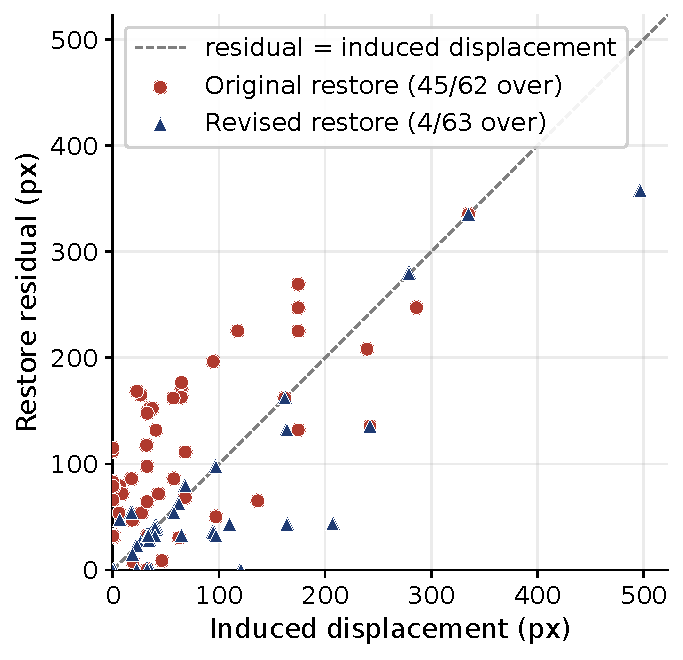
\includegraphics[width=\linewidth]{figures/eval-restore-overreposition-fixed.pdf}
  \caption{Word displacement across the 66-trial deterministic sweep: the original restore over-repositions relative to no preservation, while the revised restore holds displacement at or below the baseline.
  \draftnote{The embedded legend counts trials with measurable residuals (45/62 and 4/63); the text reports over-repositioned trials out of all 66. Reconcile the denominators against Experiments/analysis before submission.}}
  \label{fig:overreposition}
\end{figure}

\subsection{Functional Coverage and Reproducibility}

The backend's automated suite (100 tests) passes, and the build-enforced boundary test runs with it.
\draftnote{Re-run dotnet test before submission and confirm the exact test count.}
All figures and tables in this section were reconstructed from exported session records alone, using the platform's replay path rather than any live-state logging, which exercises the reproducibility claim in practice: the session record is sufficient to re-derive the evaluation.
